	\section{آشنایی با SVD}
در این بخش انتظار می رود که خواننده با مفاهیم مقدماتی در جبرخطی آشنا باشد. در صورتی که با تجزیه مقادیر تکین آشنایی دارید،‌ می توانید از این قسمت عبور کنید. برای مطالعه بیشتر می توانید به فصل ۶ \cite{matrix_methods} مراجعه کنید.
	\subsection{تعریف}
	برای هر ماتریس n $ \times $ m مانند $\mathbf{A}$که n $ \geq $ m تجزیه ای به صورت زیر وجود دارد \\
	\begin{center}
		$ \mathbf{A} = \mathbf{U} \left( \begin{array}{c} \Sigma \\ 0 \end{array} \right)\mathbf{V}^T$
	\end{center}	
	که $ \mathbf{U} \in \mathbb{R}^{m \times m} $ و $ \mathbf{ٰV} \in \mathbb{R}^{n \times n} $ متعامد و $ \mathbf{\Sigma} \in \mathbb{R}^{m \times n} $ قطری است به طوری که
	
	\begin{center}
		$ \Sigma = diag(\sigma_{1}, \sigma_{2}, \ldots, \sigma_{n}) $
		\\
		$ \sigma_{1} \geq \sigma_{2}\geq \ldots\geq \sigma_{n} $
	\end{center}

	به تجزیه بالا تجزیه SVD \LTRfootnote{singular value decomposition} گفته میشود. به ستون های $\mathbf{U}$ و $\mathbf{V}$ بردار های ویژه \LTRfootnote{singualr vectors} و به $\sigma_i$ مقادیر ویژه \LTRfootnote{singular values} گفته می شود. دقت کنید که شرط n $ \geq $ m باعث ایجاد محدودیتی در قضیه نمی شود. اگر این شرط برقرار نباشد همچنان رابطه بالا برای $\mathbf{A}^T$ وجود دارد.\\
	اثبات های متفاوتی برای قضیه بالا وجود دارد. برای دیدن اثباتی استقرایی به بخش ۱.۶ \cite{matrix_methods} مراجعه کنید.

	\pagebreak
	
	\subsection{انواع}
	تجزیه ای که در تعریف بالا ارائه شد فرم کامل \LTRfootnote{Full SVD} تجزیه SVD بود. تجزیه مقادیر تکین را به فرم های معادل متفاوتی میتوان نوشت. برای راحتی به معرفی چند فرم مختلف که در ادامه از آنها استفاده شده می پردازیم.
	\subsubsection{فرم سبک}
	\begin{center}
	$$ \drawmatrix[width= .5cm, height= 1cm] A = \drawmatrix U \times \drawmatrix[width= .5cm] {\Sigma_1}\ \drawmatrix[width= .5cm, height=.5cm] {V^T}
	$$
	\end{center}
	از آنجایی که 
	$ \Sigma_1 = \left( \begin{array}{c} \Sigma \\ 0 \end{array} \right) $
	بار قرار دادن 
	$ \mathbf{U}= \left( \mathbf{U_1}, \mathbf{U_2} \right) $
	که $ \mathbf{U_1}$  ماتریسی $ m \times n$ است، میتوان فرم بالا را به صورت زیر نوشت 
	
	
	\begin{center}
		$$ \drawmatrix[width= .5cm, height= 1cm] A = \drawmatrix[width= .5cm, height= 1cm] {U_1} \times \drawmatrix[width= .5cm, height=.5cm] {\Sigma}\ \drawmatrix[width= .5cm, height=.5cm] {V^T}
		$$
	\end{center}


	به این فرم تجزیه مقادیر تکین سبک\LTRfootnote{thin SVD} گفته می شود. 
	
توجه کنید که از آنجایی که $\mathbf{V}$ متعامد است با ضرب طرفین در $\mathbf{V}$ داریم 
	
	\begin{center}
		\begin{equation}
		\mathbf{A} v_i = u_i \sigma_i \quad i = 0, 1, \ldots, n
		\end{equation}
	\end{center}
	به طور مشابه با گرفتن ترانهاده و ضرب در $\mathbf{U}^T$ داریم 
	
	\begin{center}
		\begin{equation}
		\mathbf{A^T} u_i = v_i \sigma_i \quad i = 0, 1, \ldots, n
		\end{equation}
	\end{center}
	
	با ضرب (۱) در $ \mathbf{A^T} $ داریم 
	
	\begin{align}
		\mathbf{A^TA} v_i  & = \mathbf{A^T}u_i \sigma_i\\ \nonumber
  						   & = \sigma_i^2 v_i \nonumber
	\end{align}

    رابطه بالا نشان می دهد که $ v_i $ بردار ویژه و $ \sigma_i^2 $ مقادیر ویژه ماتریس $\mathbf{AA^T} $ هستند.\\
	به طور مشابه با ضرب (۲) در $\mathbf{A} $ داریم :
	
	
	\begin{align}
	\mathbf{AA^T} u_i  & = \mathbf{A}v_i \sigma_i\\ \nonumber
	                   & = \sigma_i^2 u_i \nonumber
	\end{align}
 	که یعنی $ u_i $ بردار ویژه و $ \sigma_i^2 $ همان مقادیر ویژه ماتریس $\mathbf{A^TA} $ هستند.\\
 	
 	\subsubsection{فرم فشرده}
 	می دانیم با ضرب یک ماتریس در ماتریسی مکوس پذیر رنک ماتریس تغییری نمی کند. در نتیجه با توجه به اینکه $\mathbf{U_1} $و $\mathbf{V} $ متعامد هستند می توان گفت 
 	\begin{center} 
 		$ \mathbf{Rank(A) = Rank(U_1\Sigma V) = Rank(\Sigma)} $
 	\end{center}
 	در نتیجه رنک ماتریس  $ \mathbf{A} $برابر با تعداد عناصر قطری ناصفر $ \mathbf{\Sigma}$ است. 
 	فرض کنید $\mathbf{Rank(A) = r} $ باشد. در اینصورت می توان تجزیه مقادیر تکین را به فرم فشرده زیر نوشت 
 	\begin{center} 
 		$ \mathbf{A = U_{m \times r}\Sigma_{r \times r} V^T_{r \times n}} $
 	\end{center}
 	به این فرم تجزیه مقادیر تکین فشرده\LTRfootnote{compact SVD} گفته میشود. دقت کنید که تجزیه فوق در صورتی که $ r \ll min\{m, n\} $ باشد باعث کاهش حجم محاسبات و فضای اشغال شده دیسک می شود.
 	
 	 \subsubsection{فرم ناقص}
 	 در صورتی که فقط از t مقدار ویژه اول ماتریس $ \mathbf{A}$ استفاده  کنیم، ‌می توان نوشت 
 	 
 	  \begin{center} 
 	 	$ \mathbf{A = U_{m \times t}\Sigma_{t \times t} V^T_{t \times n}} $
 	 \end{center}
  	به این فرم تجزیه مقادیر منفرد ناقص \LTRfootnote{truncated SVD} گفته می شود. درباره کاربرد این فرم در بخش های بعد توضیح خواهیم داد.
  	 \subsubsection{فرم ضرب خارجی}
  	 فرم سبک را می توان به صورت دیگری نیز بازنویسی کرد 

	\begin{align*}
		\mathbf{A = U_1\Sigma V^T } &= \mathbf{\left( u_1, u_2, \ldots, u_n\right)}
		\begin{pmatrix}
			\sigma_{1} & & &\\
		    & \sigma_{2} & &\\
		    & & \ddots & \\ 
		    & & & \sigma_{n} \\
		\end{pmatrix}
		\begin{pmatrix}
		v_1^T \\
		v_2^T \\
		\cdots\\
		v_n^T
		\end{pmatrix}\\
		 &= \mathbf{ \left( u_1, u_2, \ldots, u_n\right)}
		\begin{pmatrix}
		 \sigma_{1}v_1^T \\
		 \sigma_{2}v_2^T \\
		 \cdots\\
		 \sigma_{n}v_n^T
		\end{pmatrix}\\
		&= \sum_{i=0}^{n} \sigma_{i}u_iv_i^T
	\end{align*}
  	 
  		به این فرم، فرم ضرب خارجی گفته \LTRfootnote{outer product form} می شود. در این فرم ماتریس $ A $ به صورت جمع $ n $ ماتریس $ m \times n $ نوشته شده است که هر ماتریسی از مرتبه یک می باشد. در بخش 	\hyperref[sec:mat_approx]{تقریب ماتریس} از این فرم استفاده خواهیم کرد. 
  	
  	
 	
	\pagebreak
	\subsection{زیرفضا های بنیادی}
	\label{sec:fun_sub}
	\begin{itemize}
		\item{ پایه های برد } \\
	\begin{center}
	$ \mathbf{ R(A) } = \{y: y = Ax \} $ 
	\end{center}
	رابطه بالا برد ماتریس $\mathbf{A} $ است. اگر $ \mathbf{Rank(A) = r } $ با استفاده از فرم ضرب خارجی داریم 
	\begin{center}
	$\mathbf{Ax = \sum_{i=0}^{r} \sigma_{i}u_iv_i^Tx =\sum_{i=0}^{r} \left(\sigma_{i}v_i^Tx\right)u_i = \sum_{i=0}^{r}\alpha u_i } $
	\end{center}
	در نتیجه هر بردار در برد $\mathbf{A}$ را میتوان به صورت جمع $ u_i $ ها نوشت. از آنجایی که گفته شد $ u_i $ بردار هایی متعامد و در نتیجه مستقل خطی هستند می توان گفت بردار های ویژه $ u_1, u_2, \ldots, u_r $ پایه ای متعامد برای برد ماتریس $ \mathbf{A} $ است. \\
	\item{ پایه های پوچی } \\
	\begin{center}
	$ \mathbf{ N(A) } = \{x: Ax=0 \} $ 
	\end{center}
	برای هر بردار  $ z = \sum_{i=r+1}^n\beta_i v_i $ با توجه به تعامد $v_i$ ها داریم
	\begin{center}
		$\mathbf{Ax = \sum_{i=0}^{z} \sigma_{i}u_iv_i^T}\left( \sum_{i=r+1}^n\beta_i v_i \right)=0 $
	\end{center}
	از آن جایی که بعد فضای پوچی $ n - r $ است بردار های متعامد $ v_r+1, v_r+2, \ldots, v_n $پایه ای برای این فضا هستند.
	\end{itemize}
	\pagebreak
	\subsection{تقریب ماتریس}
	
	فرض کنید ماتریس $ \mathbf{A} $ ماتریسی با رنک پایین به صورت $\mathbf{A= A_0 + N} $ باشد که $\mathbf{ N }$ نویز می باشد. در این صورت اگر مقدار $ \mathbf{N} $در برابر $ \mathbf{A_0} $ کوچک باشد،‌ مقادیر ویژه $ \mathbf{A}$ رفتاری به شکل زیر دارند 
	
	\begin{figure}[h]
		\centering
		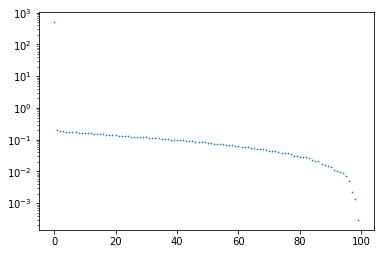
\includegraphics[width=0.7\linewidth]{assets/zero_eigenvals}
		\caption{
			مقادیر ویژه یک ماتریس بعد از اعمال نویز گاوسی با میانگین صفر و واریانس یک. ماتریس $ \mathbf{A_0} $ ماتریسی با ستون های یکسان $ 10 \times 10 $ و درایه های صحیح بین ۰ تا ۱۰ بوده. 
		}
	\end{figure}
	می توان دید که مقادیر ویژه مقداری نزدیک به صفر دارند. به تعداد مقادیر ویژه بزرگ \footnote{در اینجا به تعریفی نسبی از بزرگ بسنده می کنیم} رنک عددی یک ماتریس گفته می شود. در مسائل عملی معمولا ماتریس نویز را نداریم. اگر بتوانیم با مشاهده مقادیر ویژه رنک عددی یک ماتریس را حدس بزنیم آنگاه می توان $ \mathbf{A} $ را به صورت زیر تقریب زد. 
	\begin{center}
		$ \mathbf{A} = \sum_{i=0}^{n} \sigma_iu_iv_i^T \approx \sum_{i=0}^{k} \sigma_iu_iv_i^T $
	\end{center}
	توانستیم ماتریس  $ \mathbf{A} $ را با ماتریسی با رنک پایین تر تقریب بزنیم. این کار علاوه بر حذف نویز مزایای دیگری هم دارد. حذف مقادیر ویژه نزدیک به صفر باعث پایدارتر شدن جواب مسائل بد حالت \LTRfootnote{ ill-conditioned } می شود. بعلاوه همانطور که در ادامه خواهیم دید از این روش می توان در فشرده سازی اطلاعات هم استفاده کرد. 
	\label{sec:mat_approx}

	